\documentclass[border={20.000000bp 30.000000bp 20.000000bp 20.000000bp}, 11pt]{standalone}
\pdfinfoomitdate=1
\pdftrailerid{}
\pdfsuppressptexinfo=1
\pdfinfo{ /Creator () /Producer () }

\usepackage{tikz}
\usepackage{xcolor}
\usetikzlibrary{shapes.misc}
\usetikzlibrary{backgrounds}

\definecolor{dotColorA}{HTML}{7F7F7F}
\definecolor{dotColorB}{HTML}{7F7F7F}
\definecolor{dotColorC}{HTML}{7F7F7F}
\definecolor{dotColorD}{HTML}{BCBD22}
\definecolor{dotColorE}{HTML}{BCBD22}
\definecolor{dotColorF}{HTML}{BCBD22}
\definecolor{dotColorG}{HTML}{17BECF}

\definecolor{labelBgColorA}{HTML}{7F7F7F}
\definecolor{labelBgColorB}{HTML}{7F7F7F}
\definecolor{labelBgColorC}{HTML}{7F7F7F}
\definecolor{labelBgColorD}{HTML}{BCBD22}
\definecolor{labelBgColorE}{HTML}{BCBD22}
\definecolor{labelBgColorF}{HTML}{BCBD22}
\definecolor{labelBgColorG}{HTML}{17BECF}

\definecolor{labelTextColorA}{HTML}{FFFFFF}
\definecolor{labelTextColorB}{HTML}{FFFFFF}
\definecolor{labelTextColorC}{HTML}{FFFFFF}
\definecolor{labelTextColorD}{HTML}{FFFFFF}
\definecolor{labelTextColorE}{HTML}{FFFFFF}
\definecolor{labelTextColorF}{HTML}{FFFFFF}
\definecolor{labelTextColorG}{HTML}{FFFFFF}

\definecolor{linkColorA}{HTML}{7F7F7F}
\definecolor{linkColorB}{HTML}{7F7F7F}
\definecolor{linkColorC}{HTML}{7F7F7F}
\definecolor{linkColorD}{HTML}{BCBD22}
\definecolor{linkColorE}{HTML}{BCBD22}
\definecolor{linkColorF}{HTML}{BCBD22}
\definecolor{linkColorG}{HTML}{17BECF}

\def\textA{A New Hope}
\def\textB{The Empire Strikes Back}
\def\textC{Return of the Jedi}
\def\textD{The Phantom Menace}
\def\textE{Attack of the Clones}
\def\textF{Revenge of the Sith}
\def\textG{The Force Awakens}

\begin{document}
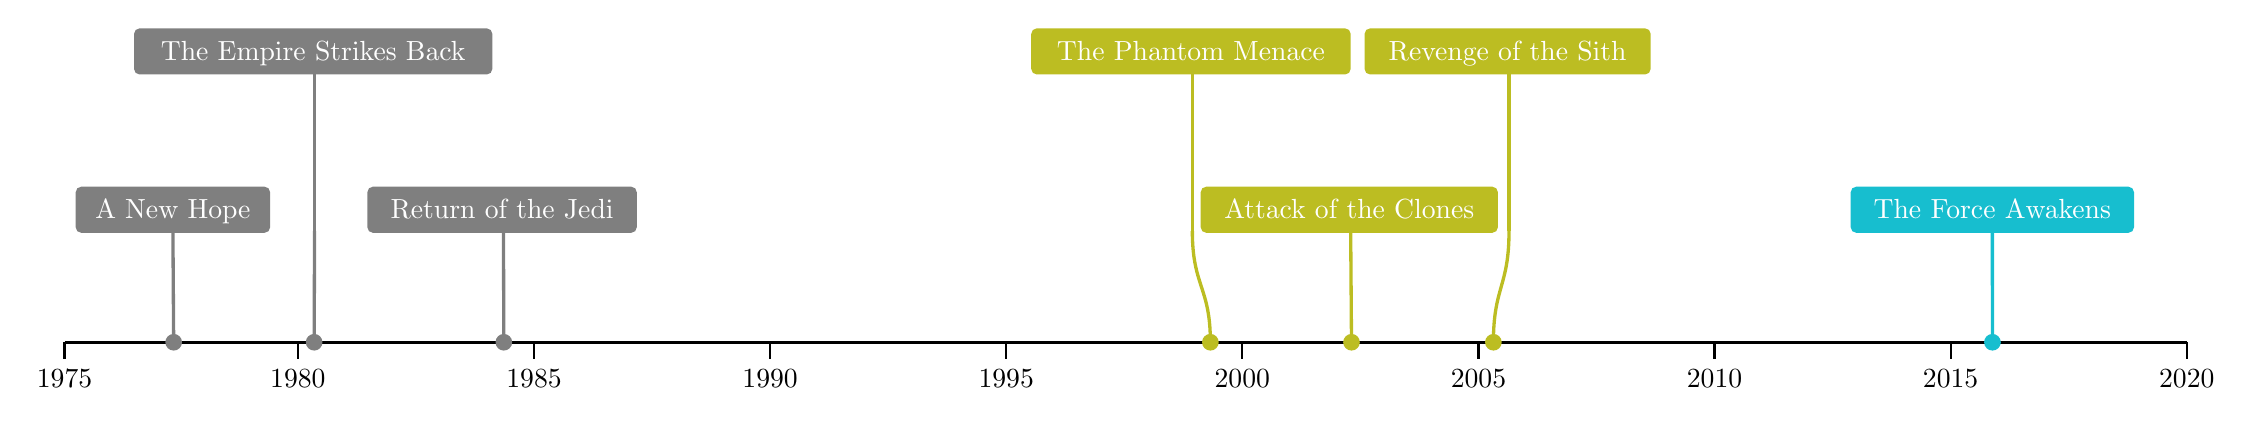
\begin{tikzpicture}[x=1bp,y=-1bp]

% shift for the margin
\begin{scope}[shift={(20, 20)}]
% main layer
\begin{scope}[shift={(0, 110)}]
% axis
\begin{scope}
\draw[very thick] (0, 0) -- (764, 0);
\end{scope}

% axis layer
\begin{scope}
\begin{scope}[shift={(0, 0)}]
\draw[thick] (0, 0) -- (0, -6pt)
node[anchor=north] {1975};
\end{scope}
\begin{scope}[shift={(84, 0)}]
\draw[thick] (0, 0) -- (0, -6pt)
node[anchor=north] {1980};
\end{scope}
\begin{scope}[shift={(169, 0)}]
\draw[thick] (0, 0) -- (0, -6pt)
node[anchor=north] {1985};
\end{scope}
\begin{scope}[shift={(254, 0)}]
\draw[thick] (0, 0) -- (0, -6pt)
node[anchor=north] {1990};
\end{scope}
\begin{scope}[shift={(339, 0)}]
\draw[thick] (0, 0) -- (0, -6pt)
node[anchor=north] {1995};
\end{scope}
\begin{scope}[shift={(424, 0)}]
\draw[thick] (0, 0) -- (0, -6pt)
node[anchor=north] {2000};
\end{scope}
\begin{scope}[shift={(509, 0)}]
\draw[thick] (0, 0) -- (0, -6pt)
node[anchor=north] {2005};
\end{scope}
\begin{scope}[shift={(594, 0)}]
\draw[thick] (0, 0) -- (0, -6pt)
node[anchor=north] {2010};
\end{scope}
\begin{scope}[shift={(679, 0)}]
\draw[thick] (0, 0) -- (0, -6pt)
node[anchor=north] {2015};
\end{scope}
\begin{scope}[shift={(764, 0)}]
\draw[thick] (0, 0) -- (0, -6pt)
node[anchor=north] {2020};
\end{scope}
\end{scope}

% link layer
\begin{scope}
\draw[color=linkColorA, very thick] (39.27647643, 0.00000000) .. controls
(39.27647643, -20.00000000) and (39.00000000, -20.00000000) .. (39.00000000, -40.00000000);
\draw[color=linkColorB, very thick] (89.85033869, 0.00000000) .. controls
(89.85033869, -20.00000000) and (90.00000000, -20.00000000) .. (90.00000000, -40.00000000);
\draw[color=linkColorB, very thick] (90.00000000, -40.00000000) -- (90.00000000, -56.60416000);
\draw[color=linkColorB, very thick] (90.00000000, -56.60416000) .. controls
(90.00000000, -76.60416000) and (90.00000000, -76.60416000) .. (90.00000000, -96.60416000);
\draw[color=linkColorC, very thick] (158.13434940, 0.00000000) .. controls
(158.13434940, -20.00000000) and (158.00000000, -20.00000000) .. (158.00000000, -40.00000000);
\draw[color=linkColorD, very thick] (412.49112720, 0.00000000) .. controls
(412.49112720, -20.00000000) and (406.00000000, -20.00000000) .. (406.00000000, -40.00000000);
\draw[color=linkColorD, very thick] (406.00000000, -40.00000000) -- (406.00000000, -56.60416000);
\draw[color=linkColorD, very thick] (406.00000000, -56.60416000) .. controls
(406.00000000, -76.60416000) and (406.00000000, -76.60416000) .. (406.00000000, -96.60416000);
\draw[color=linkColorE, very thick] (463.29740610, 0.00000000) .. controls
(463.29740610, -20.00000000) and (463.00000000, -20.00000000) .. (463.00000000, -40.00000000);
\draw[color=linkColorF, very thick] (514.38258498, 0.00000000) .. controls
(514.38258498, -20.00000000) and (520.00000000, -20.00000000) .. (520.00000000, -40.00000000);
\draw[color=linkColorF, very thick] (520.00000000, -40.00000000) -- (520.00000000, -56.60416000);
\draw[color=linkColorF, very thick] (520.00000000, -56.60416000) .. controls
(520.00000000, -76.60416000) and (520.00000000, -76.60416000) .. (520.00000000, -96.60416000);
\draw[color=linkColorG, very thick] (694.04258944, 0.00000000) .. controls
(694.04258944, -20.00000000) and (694.00000000, -20.00000000) .. (694.00000000, -40.00000000);
\end{scope}

% label layer
\begin{scope}
\begin{scope}[shift={(4, -56)}]
\fill[color=labelBgColorA, rounded corners=2pt]
(0, 0) rectangle (70, 16.60416) node[midway, yshift=-.75bp, anchor=center, text=labelTextColorA] {\strut \textA};
\end{scope}
\begin{scope}[shift={(25, -113)}]
\fill[color=labelBgColorB, rounded corners=2pt]
(0, 0) rectangle (129, 16.60416) node[midway, yshift=-.75bp, anchor=center, text=labelTextColorB] {\strut \textB};
\end{scope}
\begin{scope}[shift={(109, -56)}]
\fill[color=labelBgColorC, rounded corners=2pt]
(0, 0) rectangle (97, 16.60416) node[midway, yshift=-.75bp, anchor=center, text=labelTextColorC] {\strut \textC};
\end{scope}
\begin{scope}[shift={(348, -113)}]
\fill[color=labelBgColorD, rounded corners=2pt]
(0, 0) rectangle (115, 16.60416) node[midway, yshift=-.75bp, anchor=center, text=labelTextColorD] {\strut \textD};
\end{scope}
\begin{scope}[shift={(409, -56)}]
\fill[color=labelBgColorE, rounded corners=2pt]
(0, 0) rectangle (107, 16.60416) node[midway, yshift=-.75bp, anchor=center, text=labelTextColorE] {\strut \textE};
\end{scope}
\begin{scope}[shift={(468, -113)}]
\fill[color=labelBgColorF, rounded corners=2pt]
(0, 0) rectangle (103, 16.60416) node[midway, yshift=-.75bp, anchor=center, text=labelTextColorF] {\strut \textF};
\end{scope}
\begin{scope}[shift={(643, -56)}]
\fill[color=labelBgColorG, rounded corners=2pt]
(0, 0) rectangle (102, 16.60416) node[midway, yshift=-.75bp, anchor=center, text=labelTextColorG] {\strut \textG};
\end{scope}
\end{scope}

% dots
\begin{scope}
\draw node [circle, inner sep=0pt, minimum size=6bp, 
fill=dotColorA] at (39.276476, 0) {};
\draw node [circle, inner sep=0pt, minimum size=6bp, 
fill=dotColorB] at (89.850339, 0) {};
\draw node [circle, inner sep=0pt, minimum size=6bp, 
fill=dotColorC] at (158.134349, 0) {};
\draw node [circle, inner sep=0pt, minimum size=6bp, 
fill=dotColorD] at (412.491127, 0) {};
\draw node [circle, inner sep=0pt, minimum size=6bp, 
fill=dotColorE] at (463.297406, 0) {};
\draw node [circle, inner sep=0pt, minimum size=6bp, 
fill=dotColorF] at (514.382585, 0) {};
\draw node [circle, inner sep=0pt, minimum size=6bp, 
fill=dotColorG] at (694.042589, 0) {};
\end{scope}

\end{scope}
\end{scope}
\end{tikzpicture}
\end{document}